
\setcounter{mtc}{3} %indique le numéro réel du chapitre, pour la mini table des matières
\chapter{MISE EN SITUATION}
\minitoc  %insert la minitoc

\graphicspath{{Chapitre1/figures/}}
%==============================================================================
\pagestyle{fancy}
\fancyhf{}
\fancyhead[R]{\bfseries\rightmark}
\fancyfoot[R]{\thepage}
\renewcommand{\headrulewidth}{0.5pt}
\renewcommand{\footrulewidth}{0pt}
\renewcommand{\chaptermark}[1]{\markboth{\MakeUppercase{\chaptername~\thechapter. #1 }}{}}
\renewcommand{\sectionmark}[1]{\markright{\thechapter.\thesection~ #1}}

\begin{spacing}{1.5}

%==============================================================================
\section*{Introduction}
Avant de commencer à détailler le travail réalisé, il est indispensable d'introduire l'organisme d'accueil afin de se familiariser avec son domaine d'activité, la situation actuelle qui l'a motivé à entreprendre le projet traité au cours de ce rapport, ainsi que son orientation pour le futur.\\
Une fois entamée, nous enchaînerons avec la présentation de la problématique, suivie d'une description sommaire du sujet du projet et des concepts clés associés. Nous concluerons avec la présentation de la méthodologie de travail adoptée tout au long de la mise en œuvre du projet.


%==============================================================================
\section{Présentation de l'organisme d'accueil}

%-----------------------------------------------------------------------------------
\subsection{L'entreprise "IT SERV"}
IT SERV est une société de services et de conseil exerçant dans le domaine des Technologies de l'Information et de la Communication.
Fondée en 2008, elle a très tôt opté pour un positionnement stratégique sur les activités de conseil et de services dans le secteur des TIC en Tunisie. Elle a pour but de fournir des services à forte valeur ajoutée à ses clients. Dans ce cadre, elle vise essentiellement à les orienter vers l'adoption des technologies modernes, à maximiser l'efficacité et l'efficience de leur organisation et à optimiser leurs processus.\\
Ses valeurs fondamentales s'articulent autour de la satisfaction des clients d'une part et l'épanouissement et l'évolution de ses ingénieurs et consultants d'autre part. L'organigramme à la figure \ref{fig:organigramme} présente la hiérarchie générale de l'entreprise.\\

\begin{figure}[h]
\centering
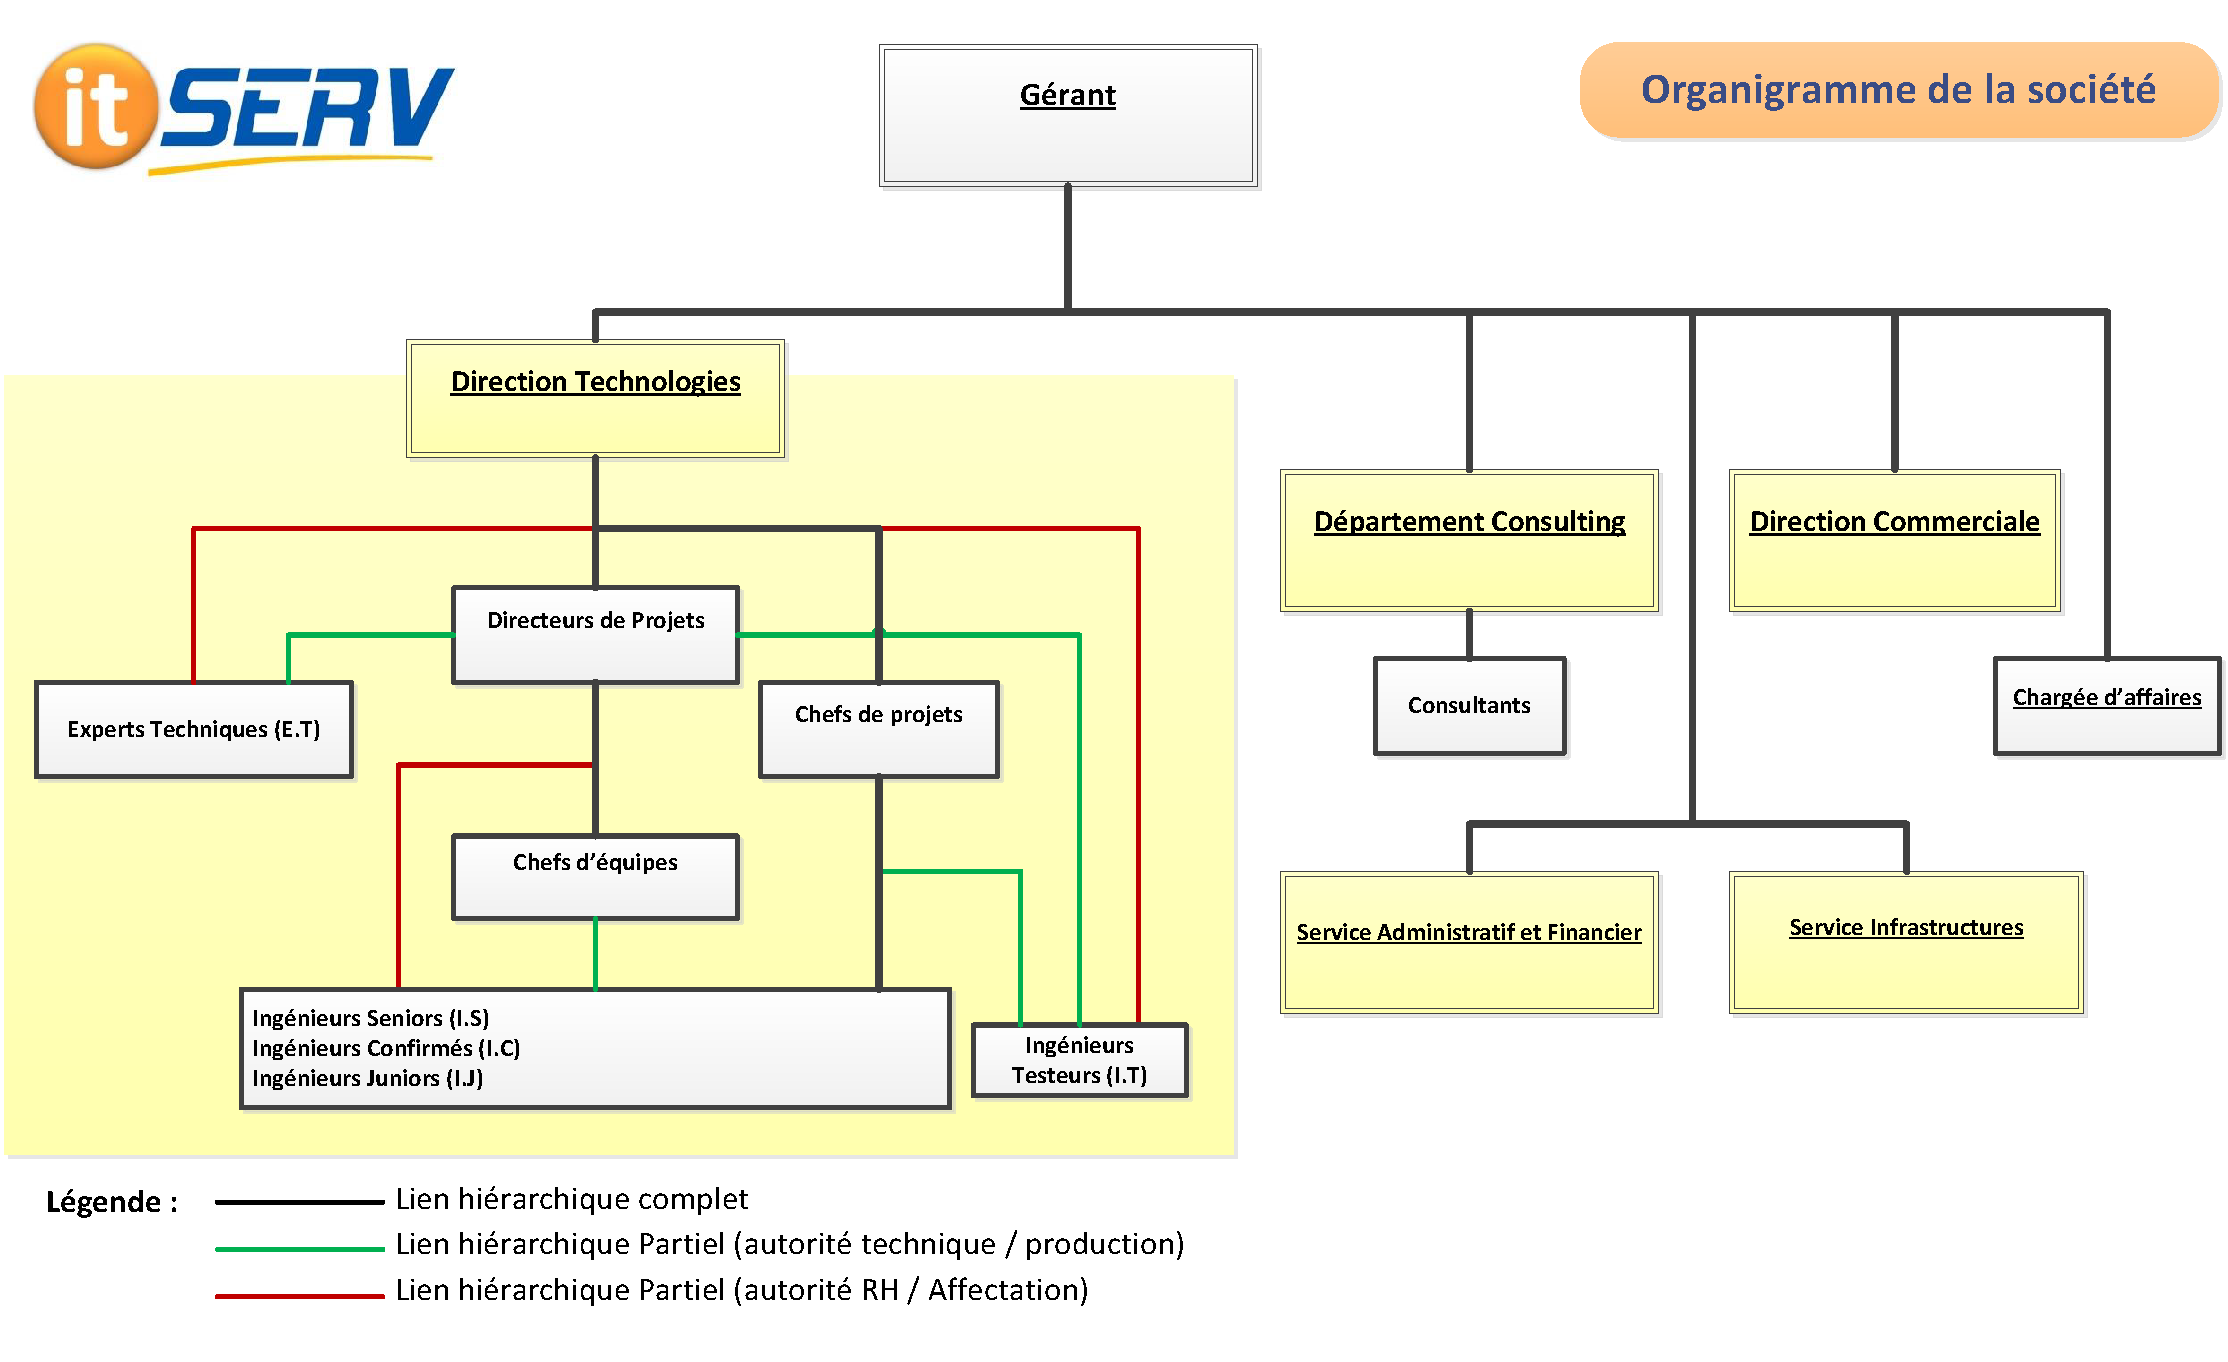
\includegraphics[width=1\linewidth]{organigramme.png}
\caption{Structure organisationnelle de l'entreprise}
\label{fig:organigramme}
\end{figure}

En plein essor, l'entreprise jouit d'une forte croissance sur tous les plans : chiffre d'affaires, résultats, effectifs, périmètre de compétence, portefeuille clients, etc. Sa réussite, à la fois en local et à l'international, constitue un facteur de stabilité et un facteur de confiance en soi pour ses clients et ses collaborateurs. Les statistiques présentées à la figure \ref{statistiquesCroissance} font le bilan des développements récents de l'entreprise.\\

\begin{figure}[h]
\centering
\includegraphics[width=0.9\linewidth]{statistiquesEntreprise.png}
\caption{Chiffre d'affaires, Croissance en nombres, Statistiques...}
\label{statistiquesCroissance}
\end{figure}

IT SERV favorise les partenariats s'inscrivant dans la continuité et la durée. En effet elle établit avec la majorité de ses clients des accords cadre, leur permettant de profiter de prix étudiés et de conditions avantageuses en matière de disponibilité, de priorité et d'engagement au plus haut niveau. Cette démarche stratégique lui permet d'avoir en contrepartie une visibilité long terme sur les commandes et les projets de ses clients, de dimensionner ses équipes en conséquence et d'optimiser son investissement en formation et mise à niveau de ses cadres en recherche \& développement.

\begin{figure}[!ht]
\centering
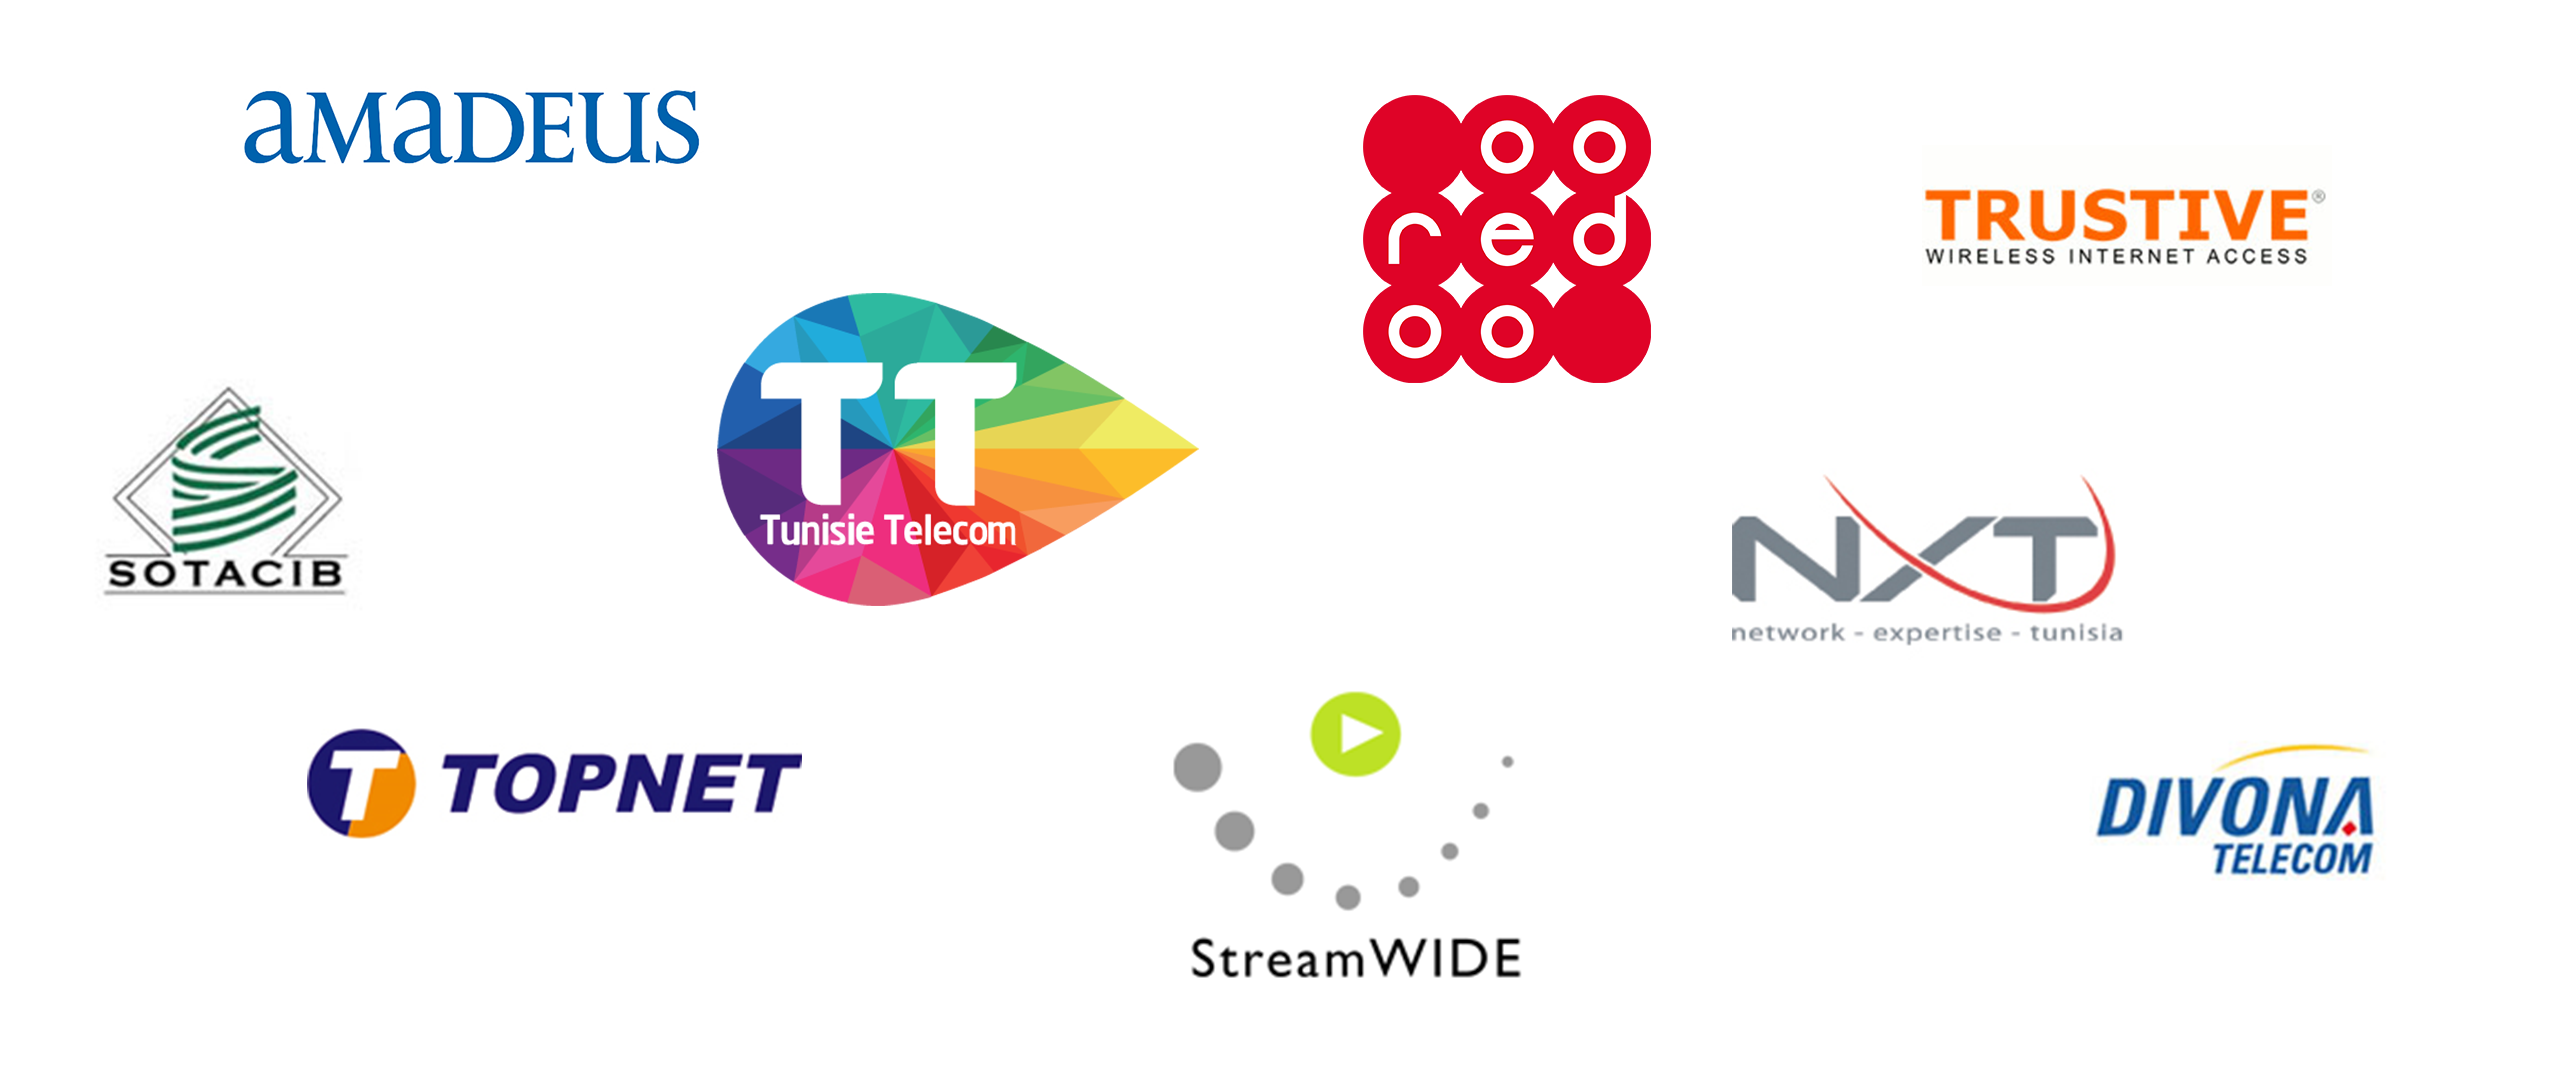
\includegraphics[scale=0.8]{references.png}
\caption{Références de IT SERV}
\label{fig:references}
\end{figure}

%-----------------------------------------------------------------------------------
\subsection{Domaine d'expertise}
L'entreprise vise la réalisation de missions complexes ayant un apport conséquent pour ses clients, dans un cadre de partenariat bénéfique pour les deux parties. La réussite de toutes ses missions et l'atteinte de ses objectifs ont instauré des relations de confiance très durables et un élargissement progressif du périmètre d'intervention.\\
\\
Les prestations d'IT SERV s'articulent autour de quatre offres :
\subsubsection*{Consulting IT} %-----------------------------------------------------------------------
IT SERV propose une large gamme de prestations de conseil stratégique, organisationnel et/ou opérationnel. L'entreprise accompagne ses clients dans la conduite du changement, la transformation de processus et la gouvernance des systèmes d’informations. Pour cela, l'offre de consulting IT se concentre autour de 3 axes d’activités :
\begin{itemize}
    \item PMO : l'entreprise propose une assistance pour la gestion efficace et efficiente des projets de ses clients. Le pilotage de projets peut porter sur l’intégralité d’un projet ou bien se focaliser sur une composante spécifique (l’initialisation du projet, la planification et le suivi de l’avancement, le suivi budgétaire et financier, etc).
    \item MOA : cette offre concerne tous les types de projets informatiques ou de télécommunications, et s’adresse à l’ensembles des secteurs et des domaines. Elle vise à aider les clients dans l’accomplissement de leurs activités de maîtrise d’ouvrage en systèmes d’information (rédaction de cahiers des charges, assistance à la sélection de fournisseurs, cadrage et assistance dans l’expression de besoins, etc).
    \item Audit : les services d’audit informatique offerts concernent à la fois les composantes organisationnelles et techniques. Ces prestations incluent l'audit des systèmes d’information (audit intégral du système d’information ou bien d'un domaine particulier) et l'audit d'applications (environnement de l’application, adéquation aux besoins fonctionnels et non fonctionnels, aux processus de l’entreprise, maintenabilité, interfaces, coût associées, etc).
\end{itemize}
\subsubsection*{Intégration \& Développement} %----------------------------------------------------------
IT SERV propose une offre complète allant du développement spécifique, à l’intégration de progiciels standards, grâce à sa connaissance approfondie des solutions du marché et la maîtrise des processus métiers de sa clientèle cible. Les prestations sont classifées selon les deux catégories suivantes :
\begin{itemize}
    \item Offres de services : conception et mise en œuvre de solutions spécifiques dans divers secteurs, intégration et interfaçage des systèmes, assistance à la migration et à la fiabilisation des données, sélection et mise en application de divers outils de management et de supervision, etc.
    \item Expertise technologique : approche méthodologique fondée sur les principes de l’agilité, mise à disposition d'architectes techniques qualifiés et à jour sur les dernières tendances technologiques, forte compétence technique sur diverses technologies (Microsoft .Net, JavaEE, Oracle, php, …), expertise dans la mise en œuvre des solutions Workflows, maîtrise parfaite des techniques d’interfaçage (ESB, Web services SOAP/REST, ETL, RPC, RMI, …), expertise en Business Intelligence, etc.
\end{itemize}
\subsubsection*{Expertise Télécoms} %--------------------------------------------------------------------
IT SERV propose ses services dans les différentes activités métiers et techniques des opérateurs, notamment : la facturation, la gestion de la relation client, le portail (Selfcare), la médiation, les programmes de fidélisation des clients, la gestion des ressources des réseaux (Network Inventory), les services à valeur ajoutée (SMS/MMS Messaging, ...), les composantes et fonctions du réseau intelligent (e-Services: e-Payment, ...), la conception de tableaux de bord et Reporting décisionnel (B.I), la ré-ingénierie de processus, etc.
\subsubsection*{Nearshore Outsourcing} %-----------------------------------------------------------------
L'entreprise se veut positionnée en tant qu’acteur de référence dans les solutions d’externalisation NearShore. Elle offre à ses clients et partenaires internationaux une solution de proximité se démarquant par une grande capacité en Nearshoring adaptée aux besoins du client et/ou partenaire, des équipes qui sont formés dans les grandes écoles Françaises et Tunisiennes, des équipes totalement francophones et parlant aussi couramment l’Anglais, une maîtrise parfaite des pratiques de l’agilité et des processus itératifs, la livraison éventuelle d’un POC afin de prouver la faisabilité de la solution proposée, ainsi qu'une conduite de projets effectuée en toute transparence avec le client (moyennant les outils adéquats).
\\

La stratégie de développement de IT SERV se repose grandement sur l’établissement de partenariats stratégiques et durables avec les acteurs locaux ou internationaux dans ses domaines d’activités. Les Partenariats établis permettent d’une part à IT SERV de disposer d’une base importante d’experts et consultants afin de répondre aux besoins actuels et futurs de ses clients, et d’une autre part, ces accords lui permettent d’accéder à des marchés nouveaux et de réaliser en collaboration avec ses partenaires des projets et missions nécessitant des expertises complémentaires et/ou des effectifs importants.
Durant les deux dernières années, plusieurs missions ont été menées dans le cadre de ces accords de partenariat.

\begin{figure}[!ht]
\centering
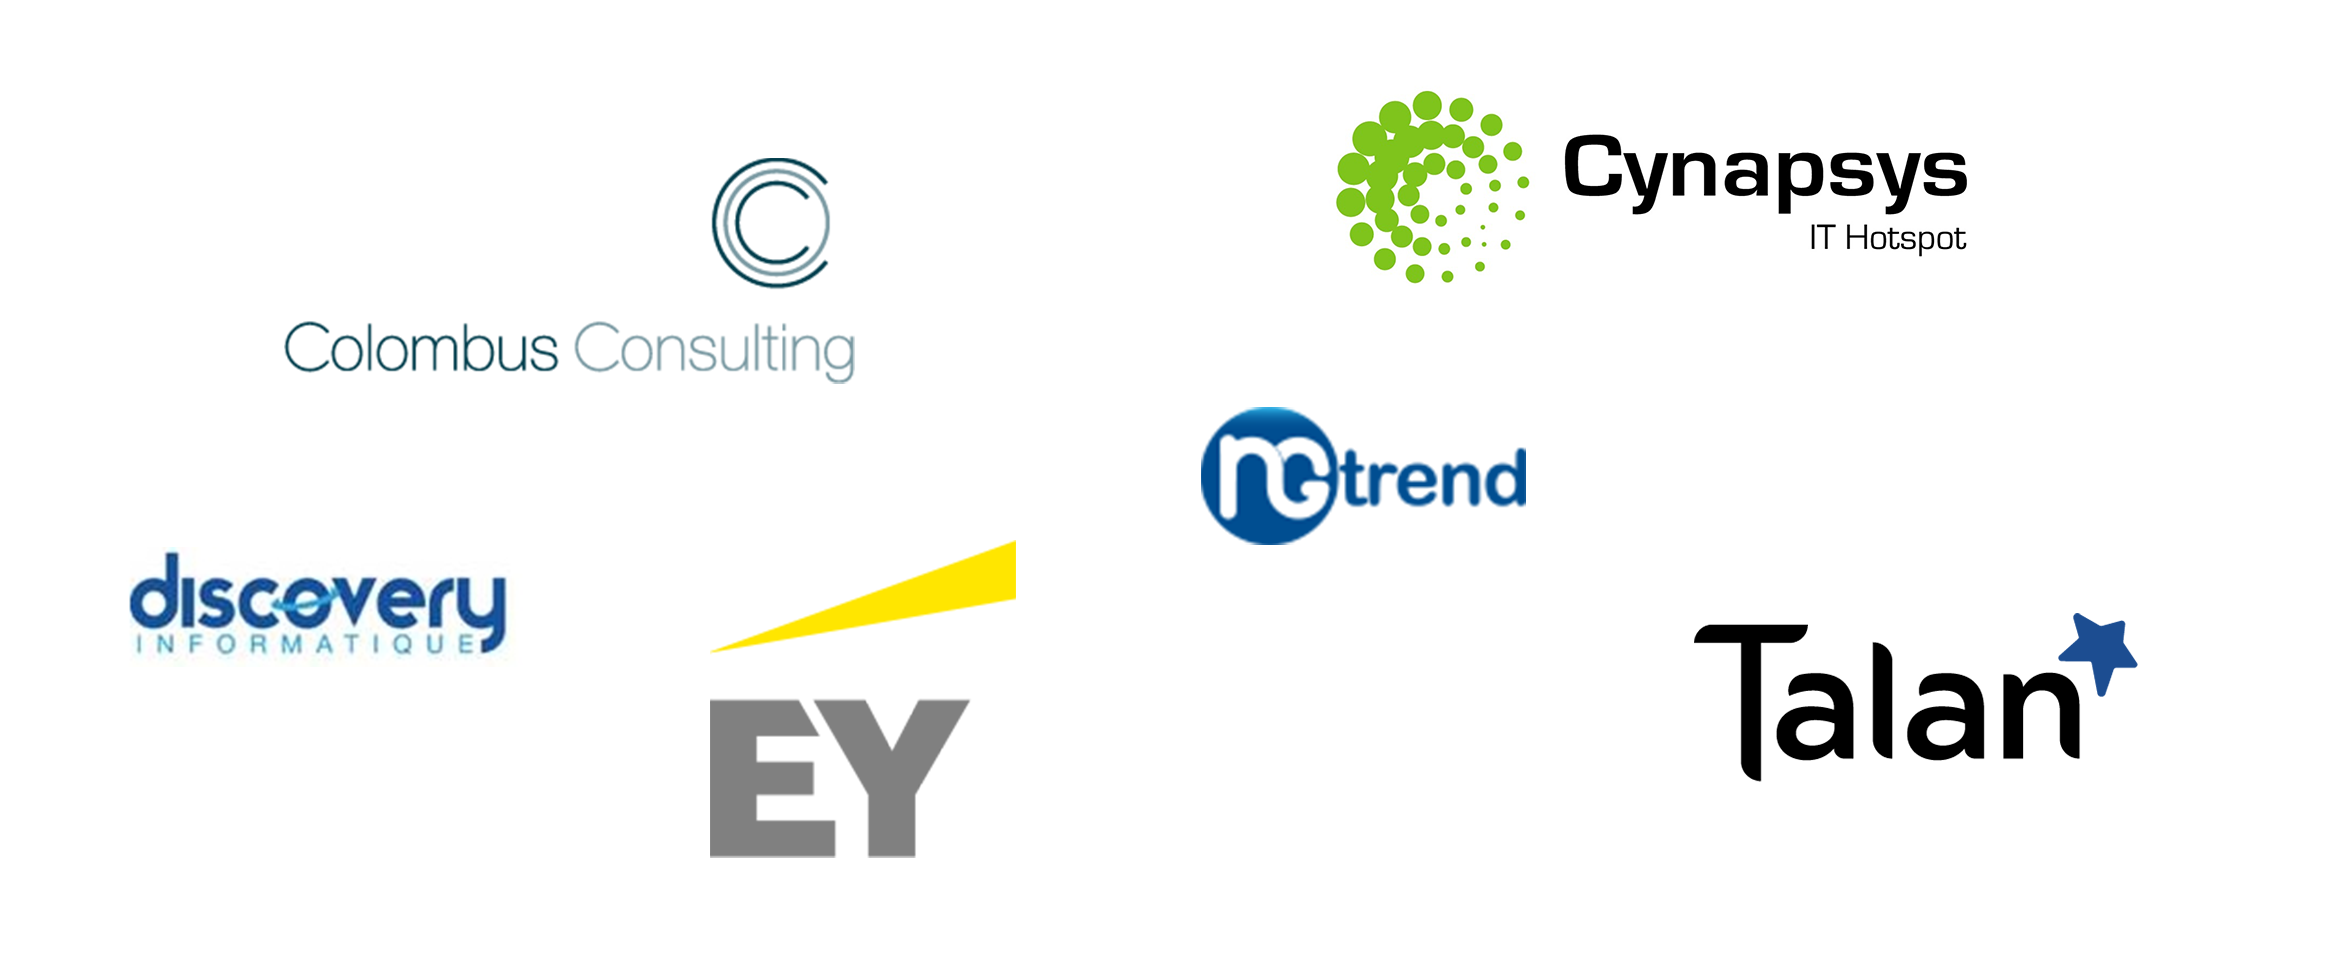
\includegraphics[scale=0.8]{partenaires.png}
\caption{Partenaires de IT SERV}
\label{fig:partenaires}
\end{figure}
\

Plus récemment, l'entreprise aspire à élargir son éventail d'offres et entrevoit de se convertir en un éditeur de logiciel à part entière.


%==============================================================================
\section{Problématique et motivations}
De nos jours, la gestion de projet s'impose dans les structures de toutes tailles comme le mode d'organisation par excellence.\\
Un projet désigne un ensemble finalisé d'activités et d'actions entreprises dans le but de répondre à un besoin, soumis à des contraintes bien définies, généralement dans des délais fixés avec une allocation budgétaire plafonnée. La gestion de projet quant à elle, représente la démarche visant à organiser de bout en bout le bon déroulement d'un projet.\\
Celle-ci revient généralement à la gestion de multiples facettes, notamment :
\begin{itemize}
\item La planification
    \item La gestion budgétaire
    \item Le pilotage des risques
    \item La gestion du changement
    \item La gestion des interventions
    \item La gestion des mises à jour
    \item La gestion des ressources
\end{itemize}
\

Avec les projets de plus en plus complexes auxquels les entreprises font face, gérer tous les flux d'information en perpétuel changement d'un projet se révèle être une tâche des plus ardues pour les chefs de projets. Sans un système efficace de traitement des données et d'achemeninement de l'information, ceux-ci finissent par être submergés par les requêtes, et se retrouvent le plus souvent dépassés par les événements. Cela se reflète en conséquence par un manquement au niveau de la réponse aux attentes de l'une ou plusieurs des parties prenantes au projet, qui, souvent dû à des contraintes de disponibilité, restent trop longtemps en déphasage avec les dernières fluctuations et les mises à jour du projet pour pouvoir prévenir les situations de crise.\\
C'est là que réside le cœur de la problématique : réussir à synchroniser de manière efficace toutes les parties prenantes à un projet avec l'état actuel de ce dernier, en distinguant le chef de projet en tant que pièce maîtresse de sa supervision.\\
\\
Le projet présent a pour but de répondre à ce problème en fournissant une solution logicielle dédiée à la gestion de projets. La solution se doit de répondre adéquatement aux attentes des chefs de projets de l'entreprise, en termes de fonctionnalités, mais aussi fournir un point pivotal d'aide à la décision pour ses dirigeants. Effectivement, les données récupérées tout au long de son exercice devront être en mesure d'être synthétisées en des données actionables, capables d'orienter les dirigeants de l'entreprise dans leur prise de décisions stratégiques quant à la détermination, entre autres,  des clients les plus profitables, les partenariats à privilégier, etc.\\
Au sein de l'environnement extrêmement concurrentiel dans lequel exerce l'entreprise, et au vu du poids dont relève sa prestation de consulting, en l'occurence LA gestion de bout en bout de projets informatiques, il est clair qu'une solution dédidée à la gestion du portefeuille de projets de l'entreprise et de ses clients constituerais un point décisif face à la concurrence, et impacterais positivement l'image de la société en influençant grandement le niveau de satisfaction de ses clients.\\

Outre l'apport de l'application pour la gestion de ses propres projets en interne, dans l'optique de sa conversion en un éditeur de logiciel, IT SERV entrevoit de développer une offre autour d'une version SaaS de l'application, depuis son propre cloud.\\
 Dans ce cadre, le développement d'une interface de gestion et de monitoring de cet aspect s'impose en tant que partie à part entière du projet. Elle se verras traîtée plus en détail au cours du chapitre \ref{chapterX}.


%==============================================================================
\section{Méthodologie de travail}
Pour la réalisation d'un projet informatique d'envergure, il est indispensable de suivre une méthodologie de travail bien établie, prenant en compte les spécificités du projet, et ce dans le but de garantir un niveau optimal de rendement tout au long de sa réalisation.

%-----------------------------------------------------------------------------------
\subsection{Choix de la méthodologie}
Les avancées majeures dans l'univers de l'informatque ont été accompagnées d'une révolution dans la manière de faire et de penser pour produire des logiciels. Celle-ci a éventuellement donnée naissance au processus unifié et au mouvement de déveoppement agile, qui se caractérisent par le développement itératif et incrémental.\\
Les deux méthodologies initialement considérées pour la mise en œuvre du projet sont RUP \cite{RUP} et SCRUM \cite{SCRUM}. Chacune met en avant les principaux avantages du processus unifié et des méthodes agiles, respectivement.\\

À première vue, le processus unifié semble assez similaire à l'approche agile. Néanmoins, il s'en distingue par certaines caractéristiques :
\begin{itemize}
\item Piloté par les cas d'utilisation et les riques
    \item Centré sur l'architecture
    \item Prescrit un niveau élévé de formalisme
    \item Préconise un travail considérable sur les spécifications en amont
\end{itemize}
Plus particulièrement, RUP s'impose en tant qu'implémentation standard du processus unifié. Son attrait majeur réside dans sa minimisation des risques très tôt dans le développement et l'adoption d'une approche rationnelle pour le cycle de développement de logiciel, scindée en quatres phases (pouvant elles-même être subdivisées en sous-itérations) :
\begin{itemize}
    \item Inception : essentiellemet, cerner le système de façon adéquate pour établir la vision, détermnier les risques et établir des prévisions (coûts, charges, ...). Si le projet ne passe pas ce jalon, il peut être annulé ou répété après avoir été réajusté
    \item Élaboration : l'objectif principal est d'atténuer les éléments de risque identifiés. C'est ici que le projet commence à prendre forme (analyse du domaine, architecture de base, ...).
    \item Construction : l'accent est mis sur le développement de composants et d'autres fonctionnalités du système. La majeure partie du codage a lieu ici
    \item Transition : transiter le système du développement à la production (bêta testing, contrôle qualité, etc)
\end{itemize}
L'approche offre une description assez élaborée du processus de développement, ce qui se révèle être très utile pour guider le développement d'une manière disciplinée et cohérente, tout en facilitant le travail de planification en aval. Cependant, cette discipline n'est pas sans prix. Le niveau de formalisme requis et la rigidité des processus prescrits pour la transition d'une phase à l'autre ainsi que pour la prise en compte du changement (planification lourde, principalement en amont, dates d'échéance, ...), nécessitant constamment la génération d'artéfacts  divers (spécifications formelles, document d'architecture, ...) la rend inadaptée à l'application au projet présent, qui nécessite de prioriser le développement rapide de fonctionnalités et la validation fréquente du rendu.\\

Les méthodes Agiles quant à elles, partent du principe que spécifier et planifier dans l’intégralité les détails d’un produit (approche prédictive) avant de le développer est contre-productif. Le terme "agile" définit une approche de gestion de projet qui prend le contre-pied des approches traditionnelles. La notion même de "gestion de projet" est remise en question au profit de "gestion de produit". De façon à raisonner davantage "produit" que "projet". Après tout l'objectif d'un projet informatique consiste bien à donner naissance à un produit \cite{http://www.agiliste.fr/introduction-methodes-agiles/}.  L’idée de l’approche consiste à se fixer un objectif à court terme et à se mettre en route sans tarder. Une fois ce premier objectif atteint, on effectue une brève revue de l'état actuel, et on adapte son itinéraire en fonction de la situation du moment, ainsi de suite, jusqu’à la destination finale.\\
 La méthode SCRUM est la méthodologie la plus utilisée parmi les méthodes agiles existantes. Elle est caractérisée par :
\begin{itemize}
    \item L’existence d’une auto-organisation
    \item Des rôles définis : Scrum Master, Product Owner, équipe de développement
    \item Un ensemble de cérémoniaux (réunion quotidienne, revue de sprint, …)
    \item La présence constante du client
    \item La mise en place de mécanismes favorisant les livraisons fréquentes (sprint, release)
    \item Une acceptation du changement (via un backlog dynamique)
\end{itemize}
La figure \ref{ScrumCycle} présente une vue d'ensemble de son cycle de vie. Cette méthode est très attractive de par son approche du développement incrémental de produit sous forme de releases (versions systèmes opérationnelles). Néanmoins, travaillant uniquement avec l'encadrant côté entreprise sur le projet présent, l'équipe de développement se résume simplement en ma personne. La mise de l'accent sur la collaboration entre les membres de l'équipe et la prescription de nombreux cérémoniaux à cet effet rend la méthode plus adaptée aux équipes plus élaborées.\\
\\
Dans le but de tirer profit des points forts de RUP tout en suivant une approche agile, s'inspirant notamment de SCRUM, nous avons choisi de suivre une méthode hybride, flexible, permettant de tirer partie des principaux attraits des approches précedemment citées : Disciplined Agile Delivery (ou l'agile discipliné). Celle-ci est présentée en détail dans la prochaine section.

%-----------------------------------------------------------------------------------
\subsection{Présentation de la méthodologie}
Disciplined Agile Delivery (DAD) est un cadre hybride qui s'appuie sur la base solide d'autres méthodes et cadres de processus logiciels. Le framework adopte des pratiques et des stratégies à partir de sources existantes et fournit des conseils pour savoir quand et comment les appliquer ensemble. Des méthodes telles que Scrum, Extreme Programming (XP), Kanban et Agile Modeling (AM) fournissent les briques de processus et DAD le mortier pour les ajuster efficacement. L'un des avantages du développement de logiciel agile et lean réside dans la richesse des pratiques, des techniques et des stratégies à disposition. C'est aussi l'un de ses plus grands défis car, sans quelque chose comme le cadre DAD, il est difficile de savoir vers lesquelles s'orienter et comment les intégrer.\\
Le diagramme \ref{fig:triphaseCycleDAD} suivant montre une vue de haut niveau du cycle de vie de la DAD. C'est un cycle de vie triphasé où l'on crée progressivement une solution consommable au fil du temps.\\

\begin{figure}[h]
\centering
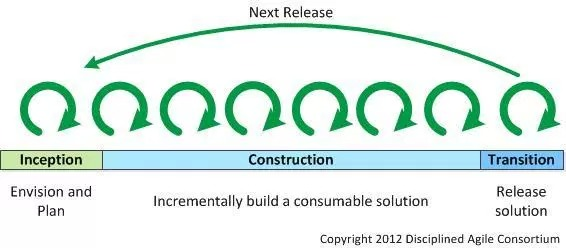
\includegraphics[width=0.8\linewidth]{triphaseCycleDAD.jpg}
\caption{Cycle de vie haut niveau de la DAD}
\label{fig:triphaseCycleDAD}
\end{figure}
\\
Évidemment, il y a à la méthode plus que montre le diagramme précedent. DAD vise à être le moins prescriptif possible et s'efforce à s'adapter et à refléter la réalité du mieux possible. Quatre propositions du cycle de vie s'en suivent :
\begin{itemize}
    \item Une version agile / basique qui prolonge le cycle de vie Scrum (Construction) avec des idées éprouvées de RUP
    \item Un cycle de vie avancé / Lean
    \item Un cycle de vie de livraison continu Lean
    \item Un cycle de vie exploratoire "Lean Startup"
\end{itemize}\\

Notre choix s'est porté sur le cycle hybride, entre RUP \& SCRUM. La figure \ref{fig:ScrumRUPcycleDAD} le présente plus en détail.
\begin{figure}[h]
\centering
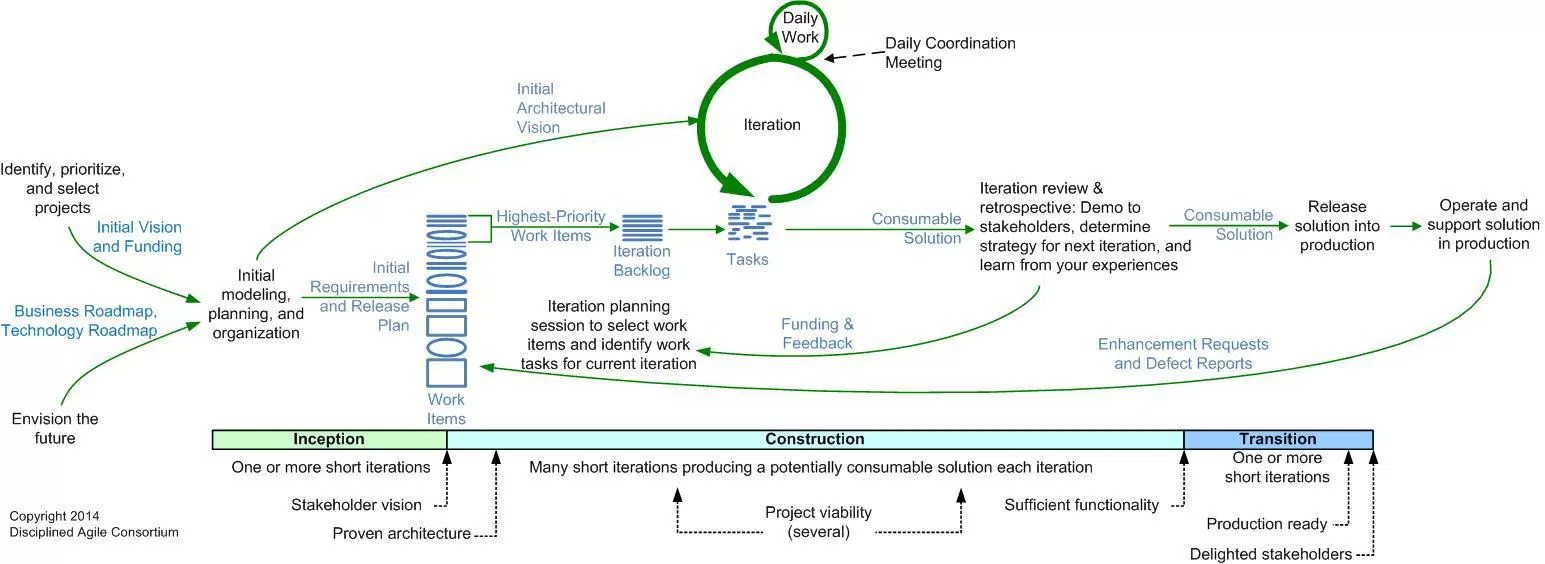
\includegraphics[width=1\linewidth]{ScrumRUPcycleDAD.jpg}
\caption{Cycle de vie basique de la DAD}
\label{fig:ScrumRUPcycleDAD}
\end{figure}

Avec DAD, nous adoptons une approche axée sur les buts. Cette approche lui permet d'éviter d'être prescriptif et donc plus souple et plus adapté à notre situation. DAD indique simplement qu'il y a plusieurs problèmes entourant un but, dont l'on doit tenir compte, et propose plusieurs techniques pratiques à envisager pour le réaliser. DAD va plus loin encore et décrit les avantages et les inconvénients de chaque technique et dans quelles situations elle convient le mieux. Il convoit que certaines options conviennent pour la plupart des cas, et les recommande généralement, tout en fournissant des alternatives pour les scénarios atypiques. Le diagramme de la figure \ref{fig:goalsDAD} indique l'ensemble des buts de haut niveau associés à chaque phase de l'approche.

\begin{figure}[h]
\centering
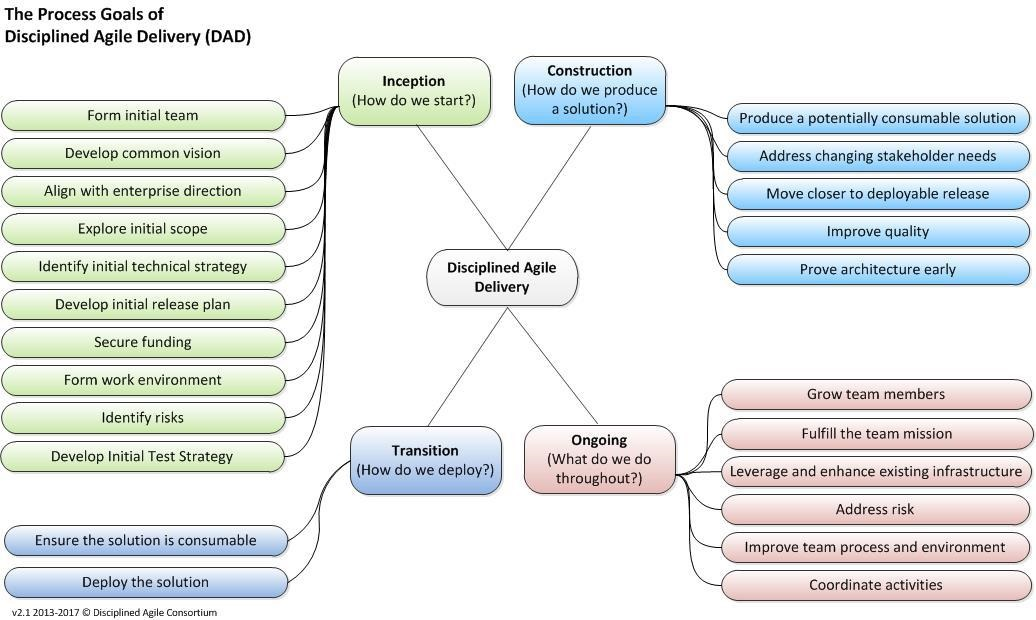
\includegraphics[width=0.95\linewidth]{goalsDAD.jpg}
\caption{Buts associés aux phases de la DAD}
\label{fig:goalsDAD}
\end{figure}

L'illustration \ref{fig:rup_scrum_dad} introduit le concept d'articles de travail ou "Work Items", assimilable au concept de Backlog de Scrum. Le Backlog faot office de carnet de fonctions, priorisées, contenant de courtes descriptions de toutes les fonctionnalités souhaitées dans le produit. La différence réside dans l'extensibilté de concept pour inclure des éléments outre fonctonnels (tel que l'élaboration de réunions, de formations, etc).\\
DAD intègre aussi un certain nombre de jalons légers, ordonnés dans le temps, dans ses cycles de vie, et ce afin de guider et de mesurer les progrès et la santé d'un projet. Ils sont dépictés en bas de la figure \ref{fig:rup_scrum_dad} :
\begin{itemize}
    \item Vision des parties prenantes : entente générale sur l'objectif du projet entre les différentes parties prenantes
    \item Architecture éprouvée : bonne pratique pour l'atténuation précoce des risques liés au bon fonctionneemnt global du système
    \item Viabilité du projet (à multiples occurences, optionnel) :  à certains moments pendant le projet, les parties prenantes peuvent demander un point de contrôle pour s'assurer que le projet progresse conformément à la vision convenue, et choisir de la mettre à jour le si nécessaire
    \item Fonctionnalité suffisante : généralement vers la fin de la phase de constrcution
    \item Prêt à la production : pour les situations non triviales, une phase de transition formelle est souvent nécessaire pour faire les préparatifs finaux dans le cadre de la livraison de la solution aux parties prenantes. À un moment donné, il faut décider que la solution est prête à être produite
    \item Parties prenantes satisfaites : les organismes de gouvernance et les autres parties sont informés quand l'initiative est officiellement terminée, afin qu'elles puissent initier une prochaine version ou diriger leurs fonds ailleurs
\end{itemize}
Le journal de travail inclut les différents jalons encontrés tout au long de l'exécution du projet.

%-----------------------------------------------------------------------------------
\subsection{Journal de travail}
Le diagramme de la figure \ref{fig:gantt} permet de visualiser l'avancement du travail effectué au fil du temps :

\begin{figure}[h]
\centering
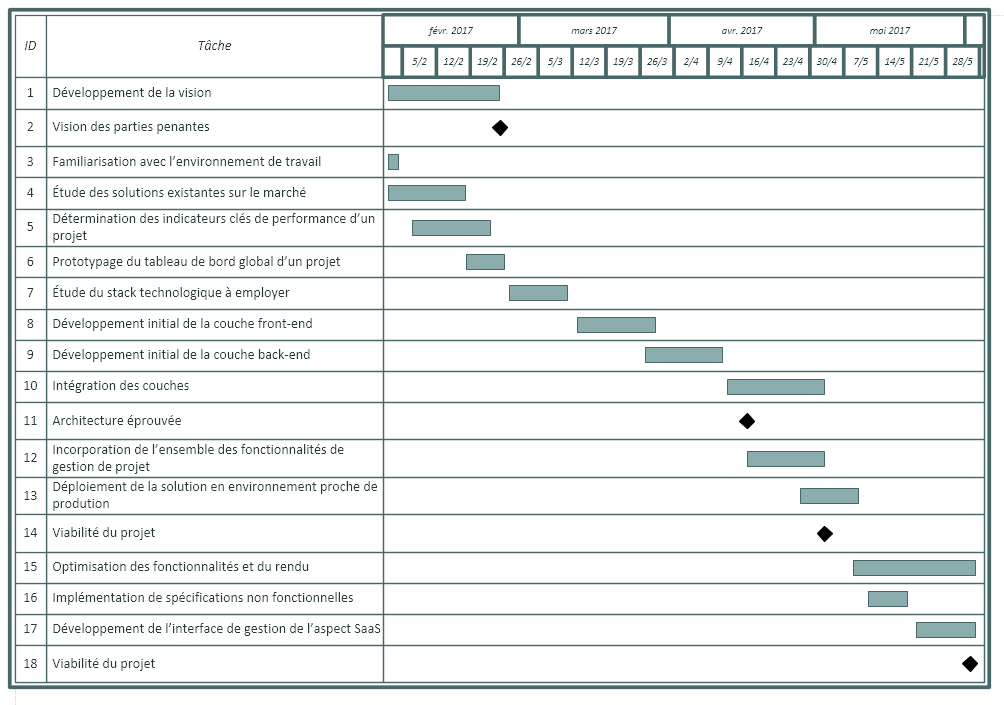
\includegraphics[width=1\linewidth]{gantt.png}
\caption{Diagramme de Gantt de l'avancement du projet}
\label{fig:gantt}
\end{figure}

%%%%% +++ Git workflow +++ %%%%%%

Le diagramme à la figure \ref{fig:gitFrontEnd} permet de visualiser l'avancement de la phase de construction au fil du temps sous forme de fréquence de commit de code :

\begin{figure}[h]
\centering
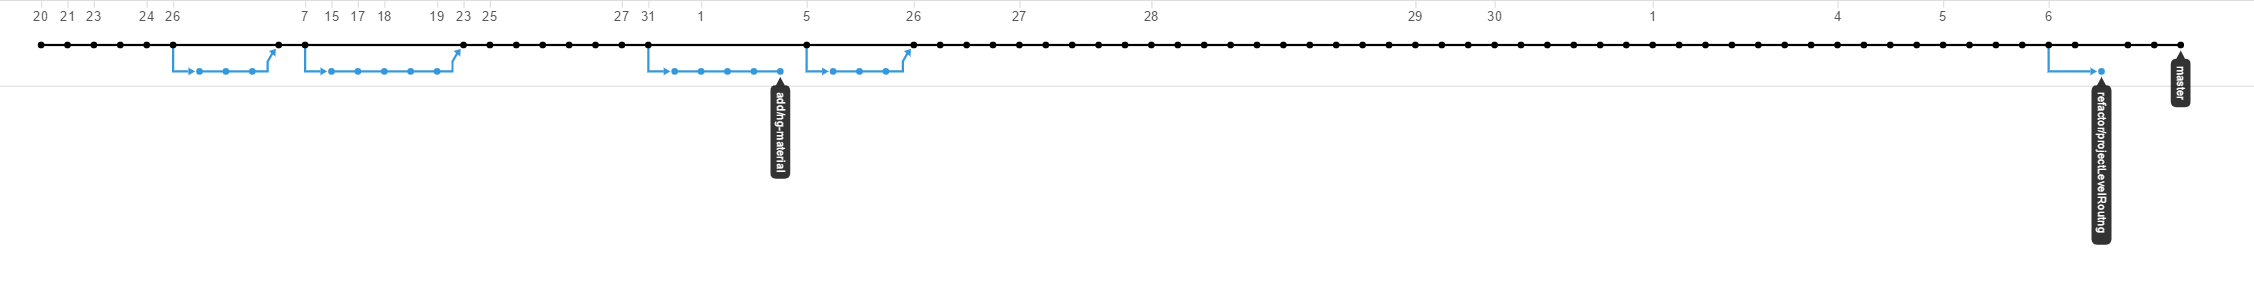
\includegraphics[width=1\linewidth]{gitFrontEnd.png}
\caption{Diagramme de commits Git}
\label{fig:gitFrontEnd}
\end{figure}

%%%%% +++ Trello Backlog peak +++ %%%%%%

%==============================================================================
\section*{Conclusion}
Dans ce chapitre, nous avons présenté le cadre général de travail, en commençant par la présentation de l'entreprise, en passant par la problématique et les motivations qui lui ont donné naissance. Pour finir, nous avons clarifié les choix méthodologiques effectués pour guider sa mise en œuvre en introduisant les concepts clés de la méthodologie de travail ainsi que des étapes effectuées tout au long de la réalisation du projet.


%==============================================================================
\end{spacing}
